	%!TEX root = ../../Main.tex
\graphicspath{{Chapters/Drivers/}}
%-------------------------------------------------------------------------------


\section{Drivers}
I dette afsnit beskrives de forskellige drivere som er lavet til projektet. 
Driverne er delt op i flere forskellige cpp filer, dette er gjort for at gøre koden mere overskuelig, og gøre funktionaliteten mere effektiv. Herunder forsøges at gøre et overblik over de forskellige cpp filer og deres integeren.  


\subsection{Display driver}
Igennem øvelser til undervisningen, er der blevet opbygget en driver til et grafisk display. Igennem processen til dette projekt er der blevet modificeret og arbejdet videre på selvsamme driver. Cpp filen ligger under TFTdriver, som er bygget op af flere forskellige funktioner. I dette afsnit vil der gives et overblik over de mest essentielle funktioner. For at få en forståelse af selve opbygningen af driveren, henvises til datasheet for controlleren. 
\href{https://blackboard.au.dk/bbcswebdav/pid-1697983-dt-content-rid-3847230_1/courses/BB-Cou-UUVA-73302/BB-Cou-UUVA-65758_ImportedContent_20170106021228/BB-Cou-STADS-UUVA-52360_ImportedContent_20160107025559/LAB/Lab3a%20Graphic%20LCD%20Display/Files%20for%20LAB3a/ILI9341_v1.11.pdf}{ILI9341} \\
For at opbygge en basisforståelse for driveren, vil der først blive forklaret DisplayInit(). Først sætter vi de porte vi skal bruge fra Arduino til hhv. indgange og udgange. Vi har dog valgt ikke at have tilbagemeldinger, og derfor er der ikke initialiseret nogle indgange. Herefter sætter vi RESET, CS, WRX, RDX høje ift figur \ref{fig:Bus_timing}. Der bliver kørt en reset (tjek lige koden med timing, burde være kortere), for at resette displayet, og bagefter sendt fire kommandoer, som kan findes i command list i databladet. Sleep Out, Display On, Pixel format set = 16 bit og Memory Access Control (BGR = 1) (Tjek ift henning hvad dette gør). 



\begin{figure}[H]
	\centering
	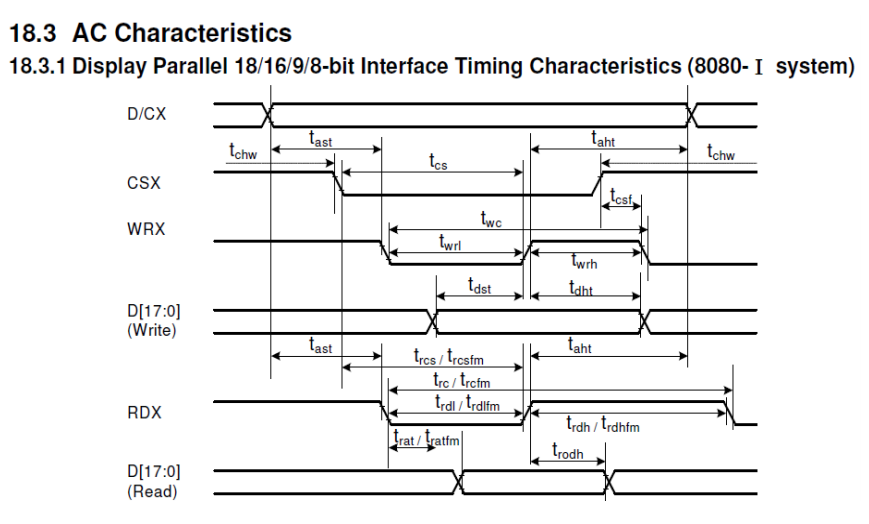
\includegraphics[width = 400 pt]{Img/Bus_timing.png}
	\caption{Bus Timing}
	\label{fig:Bus_timing}
\end{figure}

Herunder vil de essentielle funktioner deles op i hvert sin tabel. Flere af funktionerne gør brug af både Writecommand() og Writedata(), som er opbygget udfra Bus Timing figur \ref{fig:Bus_timing}. Derudover bruger flere af funktionerne SetColumnAddress() og SetPageAddress(), som er bygget op fra datasheet 8.2.20. og 8.2.21.: \\

\textbf{\Large Included Font:}

\begin{center}
\begin{tabular}{ |l|l|l| }
\hline
\multicolumn{1}{ |c| }{\textbf{character.h}} \\
\hline
Karakter størrelse: 24*24 pixels  \\
Antal karakter: 95\\
\hline

\end{tabular}
\end{center} 
\begin{figure}[H]
	\centering
	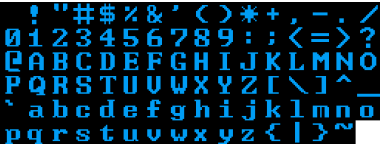
\includegraphics[width = 150 pt]{Img/Thedotfactory.png}
	\caption{The Dot Factory karakter}
	\label{fig:Thedotfactory}
\end{figure}

\textbf{\Large Funktions:}

\begin{center}
\begin{tabular}{ |l|l|l| }
\hline
\multicolumn{1}{ |c| }{\textbf{ FillRectangle(StartX,StartY, Width, Height, Red, Green, Blue)}} \\
\hline
Funktion som laver en firkant med den valgte baggrundsfarve  \\
\hline
\textbf{Paramentre:}  \\ StartX: Startværdi på x-aksen \\StartY: Startværdi på y-aksen\\ Width: Bredden på firkanten\\ Height: Højde på firkanten\\ Red: farve(værdi)\\ Green: farve(værdi) \\ Blue: farve(værdi)\\
\hline
\end{tabular}
\end{center} 

FillRectangle er en funktion som visuelt kan ændre bits til en anden farve på den givne skærm. Fra input vælges startx og starty samt længde og bredde. Derefter laves en ud fra de input der er givet. Farven afhænger også af inputtet. Det der reelt sker, er at den givne farve bliver skrevet til hver eneste pixel, i det sted der er valgt en firkant. 

\begin{center}
\begin{tabular}{ |l|l|l| }
\hline
\multicolumn{1}{ |c| }{\textbf{ drawletters(str[],startx, starty,Red, Green, Blue)}} \\
\hline
Funktion som modtager en en streng, og konverterer ascii værdien til \\den rette værdi ift character.h \\
\hline
\textbf{Paramentre:}  \\str[]: Modtager en streng\\  Startx: Startværdi på x-aksen \\Starty: Startværdi på y-aksen\\ Red: farve(værdi)\\ Green: farve(værdi) \\ Blue: farve(værdi)\\
\\

\hline
\end{tabular}
\end{center}  

drawletters er en startfunktion til drawXletter, i denne funktion, findes længden på den på det givne tegn, som skal skrives. Herudover findes lægden at det givne loop drawXletter skal fortsætte, ift hvor mange bytes der hører til det givne tegn. Denne funktion står for at finde de respektive værdier fra array\_carrier, og sende dem med til drawXletter.  til sidst sættes den nye start\_x, hvor næste tegn kan placeres, her er der valgt et mellemrum fra udvikleren på 1 pixel.

\begin{center}
\begin{tabular}{ |l|l|l| }
\hline
\multicolumn{1}{ |c| }{\textbf{ drawXletter( bitmap[],length,count,startx,starty, letter, modulus,Red, Green, Blue)}} \\
\hline
Funktion som står for at skrive til hver bit, med værdier fra letterhelper()\\
\hline
\textbf{Paramentre:}  \\bitmap[]: Henter en byte fra character.h\\ length: Fortæller funktionen, hvor bred karakteren der skal skrives er\\ count: hvor mange bytes funktionen skal køre igennem for at lave hele karakteren\\ Startx: Startværdi på x-aksen \\Starty: Startværdi på y-aksen\\ Red: farve(værdi)\\ Green: farve(værdi) \\ Blue: farve(værdi)\\
\textbf{Note:} Funktionen sletter gamle karakterer, da en ny smallere karakter end forrige stadig\\ vil forblive på displayet\\

\hline
\end{tabular}
\end{center}  

drawXletters står for at farve hver pixel, så der laves det tegn som er anmodet, dette sker ved at funktionen modtager information fra drawletters, som har information om tegn[], som er hentet fra character.h. Dette array, består af et bitmap af alle ascii tegn, og byte værdier som tegner hver pixel. Igennem funktionen sikres at bredden på tegnet overholdes, og et nyt startx punkt bliver sat, samtidig med at starty (colum) sættes til næste linje. dette gøres indtil den del af arrayet er løbet igennem som er givet fra drawletters. Til sidst i koden slettes (pixels = hvid) tegn eller pixels, som ligger forand det nye tegn som er tegnet. Dette sker for at sikre at tegnene ikke flyder ind over hinanden, hvis der findes gamle tegn på pladsen, hvor den nye tegnes. 


\subsection{Touch driver}
Da projektet skulle bruge integering af en bruger, er der valgt at inkudere en touch driver som gør brug af \href{https://blackboard.au.dk/bbcswebdav/pid-1762166-dt-content-rid-4251461_1/courses/BB-Cou-UUVA-73302/BB-Cou-UUVA-65758_ImportedContent_20170106021228/BB-Cou-STADS-UUVA-52360_ImportedContent_20160107025559/LAB/LAB10%20Touch%20Screen%20Driver/Files%20for%20LAB10/XPT2046.pdf}{XPT2046}
Touch Screen Controller, som allerede var en del af \href{https://blackboard.au.dk/bbcswebdav/pid-1762173-dt-content-rid-4251448_1/courses/BB-Cou-UUVA-73302/BB-Cou-UUVA-65758_ImportedContent_20170106021228/BB-Cou-STADS-UUVA-52360_ImportedContent_20160107025559/LAB/LAB10%20Touch%20Screen%20Driver/Files%20for%20LAB10/DS_IM120417024_ITDB02ArduinoMEGAShield.pdf}{ITDB02}
Arduino MEGA shield, som bliver også bliver brugt i Display driveren. \\
Driveren har tre funktioner, hvor Init() sætter de forskellige porte til hhv indgange og udgange, og derefter sætter de respektive ben til enten høj og lav. Funktionen pulse() står for at lave en puls på clk benet som er opsat ift. Figur 15 i \href{https://blackboard.au.dk/bbcswebdav/pid-1762166-dt-content-rid-4251461_1/courses/BB-Cou-UUVA-73302/BB-Cou-UUVA-65758_ImportedContent_20170106021228/BB-Cou-STADS-UUVA-52360_ImportedContent_20160107025559/LAB/LAB10%20Touch%20Screen%20Driver/Files%20for%20LAB10/XPT2046.pdf}{XPT2046}
datasheet. 
Herunder vil der laves en tabel over den sidste funktion. 

\begin{center}
\begin{tabular}{ |l|l|l| }
\hline
\multicolumn{1}{ |c| }{\textbf{TouchRead(xy)}} \\
\hline
Funktion som står for at læse værdien fra brugerinputtet.\\
\hline
\textbf{Paramentre:}  \\ xy: Styrer om retur værdien skal være for x eller y \\
\textbf{Retur:} Værdien for enten x eller y. \\
\\

\hline
\end{tabular}
\end{center}  

TouchRead står for at læse den værdi som bliver sendt over en seriel linje fra touch controlleren. Denne værdi skal ligges korrekt ind i en int, og bliver lagt en til hver bit, hvor gang der modtages ettal på PINE bit 5, herefter retuneres int værdien. 


\subsection{Bluetooth modul}

Bluetooth-modulet der bliver brugt i BA-TA systemet er af typen HC-05. Denne type-version understøtter nemlig mulighed for at tage rollen som både Master/Slave i et Bluetooth Master/Slave forhold imellem to parrende Bluetooth-enheden. Bluetooth modulet er sammensat med et breakout- board i bunden af modulet, hvilket giver nem adgang til de brugbare pins på selve Bluetooth-modulet, hvilket også kan ses på figur \ref{fig:bluetooth_modul}

\begin{figure}[H]
	\centering
	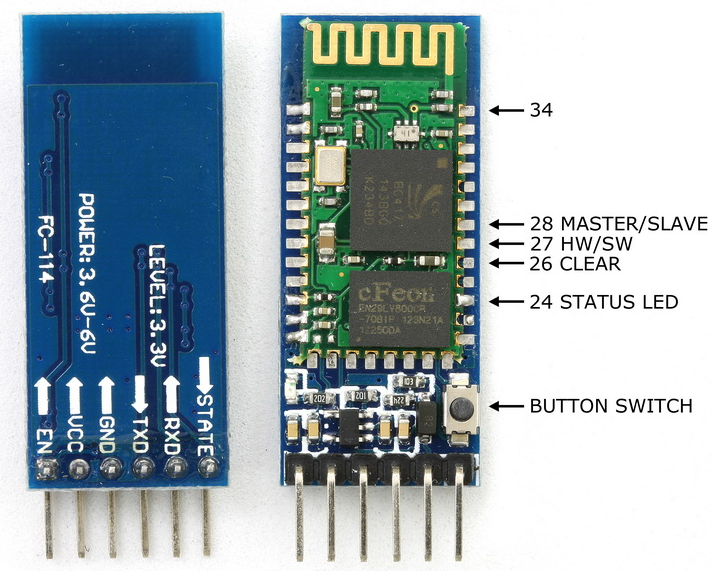
\includegraphics[width = 200 pt]{Img/modul.PNG}
	\caption{Bluetooth modulet: HC-05 GW-040.}
	\label{fig:bluetooth_modul}
\end{figure}

\subsubsection{Protokol}
Der kommunikeres til systemets Bluetooth-modul igennem en UART-forbindelse. Gruppens implementerede UART-driver på Arduino’en gør det muligt, at Arduinoen og Bluetooth-modulet kan kommunikere sammen vha. AT-kommandoer. 
AT-kommandoerne (Attention-commands) som Bluetooth-modulet understøtter kan bruges til generel opsætning af modulet, sætte Master/Slave roller, scanne for nærtliggende Bluetooth-enheder, samt at spørge om navn på fundne Bluetooth-enheders adresser. AT-kommandoerne er en general standard som bruges til at sende instruktioner til et modul og dermed er de opbygget på samme måde for hvert modul der bruger dem. På en etableret UART forbindelse vil man kunne sende en ”AT+kommando” til modulet, hvorefter modulet vil udføre kommandoen, og evt sende et svar tilbage, samt et OK, hvilket indikerer at beskeder var succesfuldt modtaget af modulet. Det samme er gældende for HC-05 Bluetooth modulet som indgår i BA-TA systemet.
Eksempler på brugte AT-kommandoer til Bluetooth-modulet i BA-TA:

\begin{itemize}
	\item ”AT+INIT” – Initialisering af Bluetooth-modulets Bluetooth SPP profil
	\item “AT+INQM,0,5,4” – Sætter scanner parameter. I dette tilfælde at der maksimum skal findes 5 Bluetooth enheder og at timeout på en scanning af Bluetooth enheder er 4*1.28 sekunder.
	\item ”AT+RNAME?<indsæt,Adresse,Her>” – Bluetooth-modulet spørger om navnet på adressen til den respektive indsætte adresse.
\end{itemize}

En succesfuld AT-kommando vil altid få Bluetooth-modulet til at returnere et OK. Såfremt der eksempelvis bliver spurgt om et navn på en respektiv Bluetooth-enheds adresse, så vil Bluetooth-modulet også returnere den fundne Bluetooth-enheds navn og et OK til sidst. 

\begin{figure}[H]
	\centering
	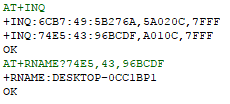
\includegraphics[width = 200 pt]{Img/uart_eksempel.PNG}
	\caption{Kommunikationseksempel med AT-kommandoer ved brug af en UART forbindelse til Bluetooth modulet.}
	\label{fig:UART_eksempel}
\end{figure}

På ovenstående figur,  \ref{fig:UART_eksempel}, kan vi se et eksempel på kommunikation vha. en UART forbindelse til Bluetooth modulet. I eksemplet bliver der sendt et "AT+INQ" til Bluetooth-modulet. Denne besked betyder inquiry, og derfor går Bluetooth modulet straks igang med at undersøge hvilke nærtliggende Bluetooth enheder den kan finde. Herefter svarer den tilbage med et "+INQ:<AdressePåFundetEnhed>" hver gang den har fundet en ny enhed. Dette forsætter den med indtil den når sit maks antal devices eller timeout grænse, som er bestemt af kommandoen "AT+INQM". Når timeout eller maks antal enheder er nået returnerer Bluetooth modulet også et OK for at indikere at den er færdig. Herefter er den også klar igen til at modtage nye beskeder.

\subsubsection{Implementering}

Da AT-kommandoerne og retur-beskederne er opbygget med samme struktur, har gruppen med fordel taget brug af dette til, at kunne udvikle en Bluetooth-kommunikations-driver, som netop udnytter denne gentagende og genkendelige proces. 

\begin{figure}[H]
	\centering
	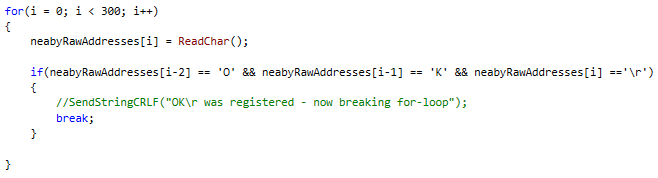
\includegraphics[width = 400 pt]{Img/OK_registrered.PNG}
	\caption{Registrering af det returnede "OK" fra Bluetooth modulet}
	\label{fig:OK_registrered}
\end{figure}

På figur \ref{fig:OK_registrered} kan vi se et eksempel på, hvordan gruppen har udnyttet at der altid vil blive sendt et OK retur til sidst, når Bluetooth modulet indikerer at den er færdig med den instruktionen/kommandoen som den har modtaget forinden. I eksemplet fra figuren benytter gruppen sig af dette til at tjekke hvornår Bluetooth modulet har sendt alt information om Bluetooth enheders adresser, som den har registreret ved sit "AT+INQ".

\begin{figure}[H]
	\centering
	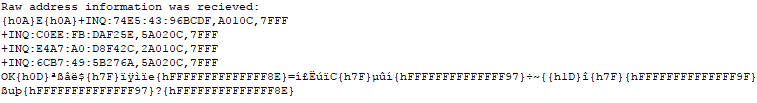
\includegraphics[width = 500 pt]{Img/raw_address.PNG}
	\caption{Al rå adresse information modtaget fra Bluetooth modulet}
	\label{fig:raw_address}
\end{figure}

Herefter kan der analyseres på det char array som alt adresse information for alle fundne enheder ligger i. Formålet med dette er at få skilt informationen ad således vi tage separere de forskellige adresser fra hinanden. Dette skyldes at dataen i det pågældende char array højst sandsynligt er loaded med flere adresser, som det eksempelvis kan ses på figur \ref{fig:raw_address}

Næste skridt er hermed at skille alt den information vi får udover MAC-adressen til de bestemte enheder. Dette gøres ved brug af "delimeter" princippet. Delimeter princippet kan bruges i dette tilfælde, da alle modtagede adresser i char array'et er sammensat og seperaret fra hinanden på en kontinuerlig måde. Hver MAC-adresse starter efter "+INQ:, de 3 dele af MAC adressen er separeret af ":" og MAC-adressen slutter ved et ",". Dette kan også ses på figur \ref{fig:raw_address}.


\begin{figure}[H]
	\centering
	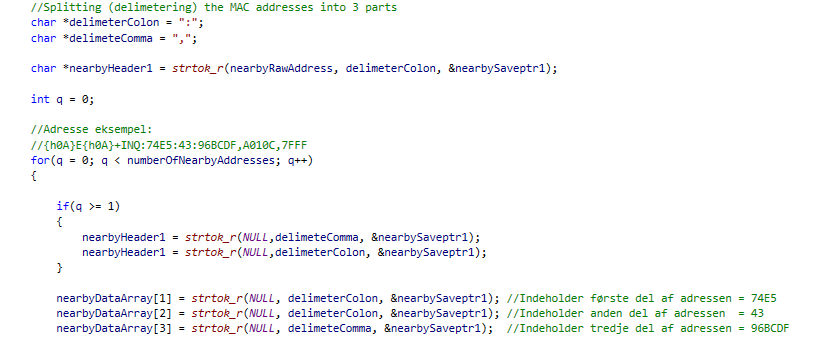
\includegraphics[width = 500 pt]{Img/delimetering.PNG}
	\caption{Brug af "delimeter"\-princippet ved brug af strtok\_r funktionen}
	\label{fig:delimeter}
\end{figure}

På ovenstående figur, \ref{fig:delimeter}, kan vi se det "delimeter"-princippet som er taget i brug for at kunne skære alt andet end de 3 dele af adressen (i dette tilfælde, 74E5, 43 og 96BCDF).

Herefter skal addressen nemlig sammensættes på en ny måde, således at vi kan få Bluetooth modulet til at spørge adressens respektive Bluetooth enhed om enhedens navn. Dette er en nødvendighed for at kunne vise navnet til brugeren i brugergrænsefladen i use case 1 og use case 2.

Før at Bluetooth modulet kan registrere at systemet forespørger navnet på en fundet Bluetooth enhed, og dens respektive adresse, skal det dermed følge denne form:\\ "AT+RNAME?74E5,43,96BCDF" og ikke:\\ "AT+RNAME?74E5:43:96BCDF", som vi modtog adressen i første omgang fra Bluetooth modulet. Forskellen er ikke stor, men udbytningen af koloner til kommaer er forskellen på om Bluetooth modulet kan genkende og eksekvere kommandoen den modtager. Dermed har der været et implementeringsbehov for at kunne tage højde for dette. Dette tager resten af koden i funktionerne addressDelimeter og trustedAddressDelimeter sig af. Forskellen på disse to funktioner er at den ene bruges til at gøre det for de enheder som skal på den godkendte liste over Bluetooth enheder i systemet. addressDelimeter bruges derimod til når låse staten er sat til auto, da funktionaliteten i de 2 funktioner varierer i forhold til hinanden.

\textbf{*** HVIS DER ER PLADS TIL MERE TEKST KAN NAVNE-FUNKTIONEN GODT UDDYBES HER}

\subsection{SystemMaster}
Dette driver/modul, står for at forbinde de andre cpp filer, og for at køre systemets funktionalitet. Derfor kaldes denne klasse også for master, da den fungerer som master ift. de andre klasser, som derved er slaves. Ift \textbf{REF TIL ENTITY}, ses Touch.h ikke som implementeret i denne klasse. Dette skulle den have været, men pga tidspres blev dette nedprioteret, derudover skulle klassen counting\_millis.c også være implementeret, mere om det i afsnittet Tekniske overvejelse og valg. 
Heruder vil kort gives et overblik over koden:
\newline
\newline
Strukturen i koden er bygget op af forksellige states, som systemet kan komme i. I hver state, bruges flere forskellige funktioner, for at skabe det display som vist i afsnittet Brugergrænseflade. På figur \ref{fig:dafaultkode} vises
et udklip fra dafault staten, som laver Hoved Menuen fra afsnittet Brugergrænseflade. 
\begin{figure}[H]
	\centering
	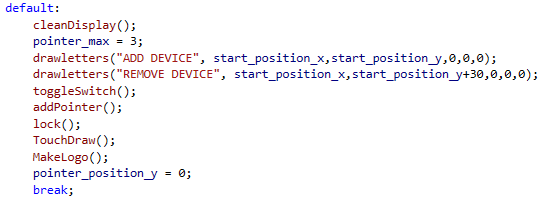
\includegraphics[width = 300 pt]{Img/dafaultkode.PNG}
	\caption{Koden til default staten}
	\label{fig:dafaultkode}
\end{figure}

Funktionaliteten fungerer på den måde at hvis auto mode sat i Hoved Menuen, vil der tjekkes for gemte enheder ift nye adresser som modtages fra bluetooth modulet. Det forløbige produkt, har en update state, som vises når den opdaterer nye værdier, og derved ikke kan brugeren ikke integere med systemet samtidig. Dette vil blive yderligere forklaret i afsnittet Tekniske overvejelse og valg. 